\documentclass{beamer}
% \documentclass[notes]{beamer}

\usepackage{graphicx}       % Extended support for \includegraphics
\usepackage{tikz}           % Powerful drawing package, part of pgf
\usepackage{url}            % \url command for decent line breaks in urls
\usepackage{array}          % Improved array support
\usepackage{textcomp}       % Extra symbols

% Enable this for summary printout
% \usepackage{pgfpages}\pgfpagesuselayout{4 on 1}[
%     a4paper, landscape, border shrink=2mm]


\usetikzlibrary{matrix}             % Grid placement
\usetikzlibrary{positioning}        % Anchor placement support
\usetikzlibrary{calc}               % Coordinate calculations
\usetikzlibrary{shapes.geometric}   % cylinder
\usetikzlibrary{shapes.symbols}     % cloud
\usetikzlibrary{shapes.arrows}      % arrow shapes
\usetikzlibrary{shapes.multipart}
\usetikzlibrary{fit}                % Fitting outline to shape
\usetikzlibrary{shadows}
\usetikzlibrary{arrows}
\usetikzlibrary{chains}

% Common TikZ definitions
\tikzset{
    % This seems a reasonably comfortable arrow shape
    >=stealth,
%
    % Used for creating an exact fit to an existing list of objects
    tight fit/.style={fit=#1, inner sep=0, line width=0},
%
    % Draws a reasonably sensible looking disk icon
    disk icon/.style={
        draw, thick, cylinder, shape border rotate=90,
        minimum width=1cm, minimum height=.75cm},
%
    % A moderate highlighting fill
    background fill/.style={fill=black!15},
    % A gentle highlighing fill
    highlight fill/.style={fill=green!60!blue!20},
    % A rather darker fill for shadows
    shadow fill/.style={fill=gray}}

% It's handy to have a foreground and background layer available.
\pgfdeclarelayer{background}
\pgfdeclarelayer{foreground}
\pgfsetlayers{background,main,foreground}


\usetheme{dlstalk}
\setbeamertemplate{navigation symbols}{}
\setbeamertemplate{items}[circle]

\hyphenpenalty 4000 \sloppy

% \title{A new Fast Data Logger and Viewer at Diamond:\\the FA Archiver}
\title[The FA Archiver]{A Fast Acquisition Archiver}
\author{Michael Abbott}
\date{Controls Group Technical Seminars\\ 25th July 2012}




\begin{document}

\begin{frame}\frametitle{Forthcoming Controls Seminars}

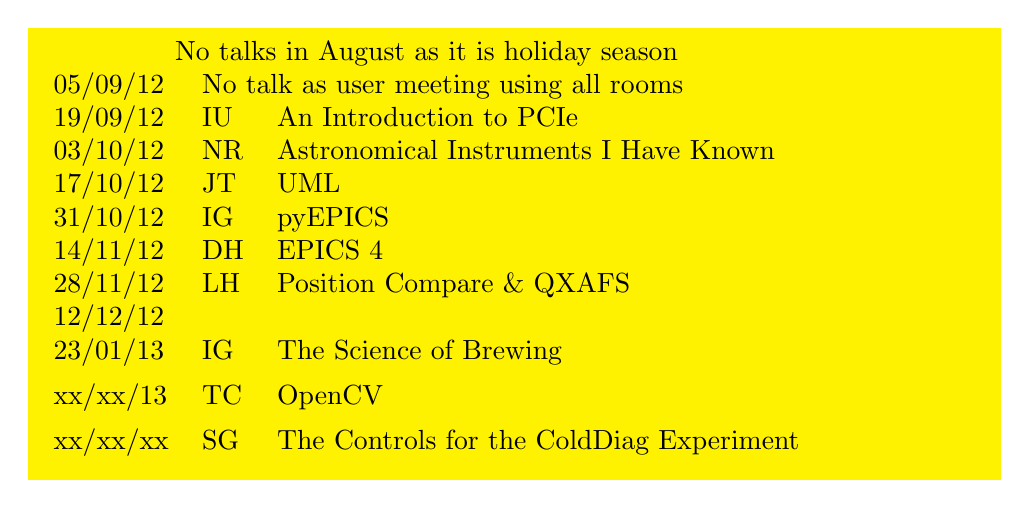
\begin{tikzpicture}
\node [fill=yellow] {
\begin{tabular*}{\textwidth}{lll}
\multicolumn{3}{c}{No talks in August as it is holiday season} \\
05/09/12 & \multicolumn{2}{l}{No talk as user meeting using all rooms} \\
19/09/12 & IU & An Introduction to PCIe \\
03/10/12 & NR & Astronomical Instruments I Have Known \\
17/10/12 & JT & UML \\
31/10/12 & IG & pyEPICS \\
14/11/12 & DH & EPICS 4 \\
28/11/12 & LH & Position Compare \& QXAFS \\
12/12/12 \\
23/01/13 & IG & The Science of Brewing \\[1ex]
xx/xx/13 & TC & OpenCV \\[1ex]
xx/xx/xx & SG & The Controls for the ColdDiag Experiment \\[1ex]
\end{tabular*}
};
\end{tikzpicture}

\begin{small}
\color{red}
Volunteers to present future seminars from December 2012 are required.

\color{blue}
Please contact James O'Hea or Mark Heron with a proposed topic.
\end{small}
\end{frame}


\begin{frame}
\titlepage
\end{frame}

% Place date discreetely on every slide.
\setbeamertemplate{footline}{\hspace*{\fill}\insertdate}


\begin{frame}\frametitle{The Fast Acquisition Archiver}

The FA archiver captures $X,Y$ position data from a network of electron beam
position monitors (EBPMs) and other sources at 10\,kHz, maintains a rolling
historical record and rebroadcasts the complete data stream to all interested
parties.

\begin{itemize}

\item Up to 512 $X,Y$ position updates every 100\,\textmu s, sustained data
rate of 40\,MB/s.

\item Current we archive the last 2\textonehalf{} days of orbit position, with
the new 30TB archiver we'll have a fortnight of archive available.

\item Any number of clients (limited by network connection to archive server)
can read the archive and subscribe to the rebroadcast live data stream.

\end{itemize}
\end{frame}



\begin{frame}\frametitle{The Fast Acquisition Archiver}
\begin{center}
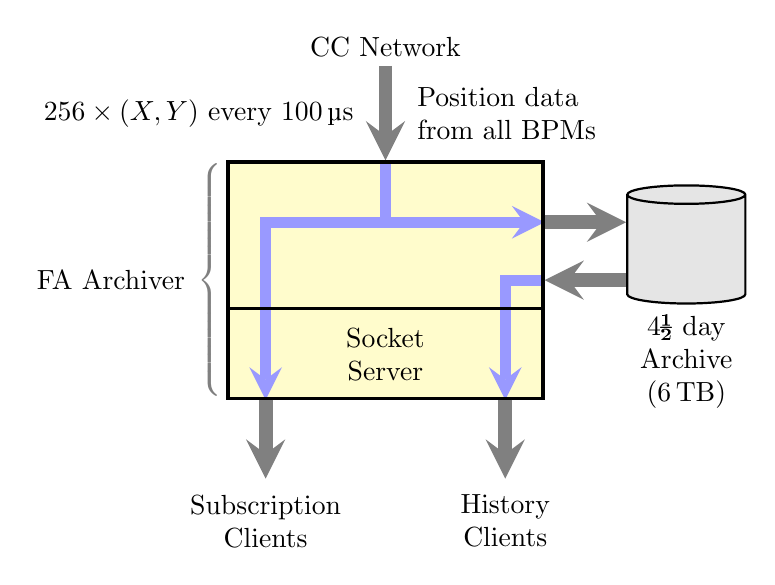
\begin{tikzpicture}

\tikzset{
    accent/.style={color=blue!40, line width=4pt},
    highlight/.style={fill=yellow!20}}

\path (0,0)
    node (cc) {CC Network}
    [draw, line width=5pt, gray, ->] (cc.south) -- ++(0,-12mm)
    coordinate (input)
    node [midway, left, black, xshift=-2mm]
        {$256\times(X,Y)$  every 100\,\textmu{}s}
    node [midway, right, black, align=left, xshift=2mm]
        {Position data\\from all BPMs};
\node (archiver) [
        draw, very thick, rectangle, anchor=north,
        label={[xshift=-4mm]left:FA Archiver},
        minimum width=40mm, minimum height=30mm] at (input) {};
\path [gray] node [fit=(archiver), inner sep=0pt, left delimiter=\{] {};

\draw[very thick] (archiver.-10) -- (archiver.-170);
\path (archiver.-10) -- (archiver.south west)
    node [midway, align=center] {Socket\\Server};

\draw [line width=5pt, gray, ->] (archiver.-135) -- +(0, -10mm)
    node [black, anchor=north, align=center] {Subscription\\Clients};
\draw [line width=5pt, gray, ->] (archiver.-45) -- +(0, -10mm)
    node [black, anchor=north, align=center] {History\\Clients};

\begin{pgfonlayer}{background}
\path[highlight] (archiver.north west) rectangle (archiver.south east);
\draw[accent, ->] (archiver.north) |- (archiver.20);
\draw[accent, ->] (archiver.0) -| (archiver.-45);
\draw[accent, ->] (archiver.north |- archiver.20) -| (archiver.-135);
\end{pgfonlayer}

\node (disk) [disk icon, fill=black!10,
    minimum height=15mm, minimum width=15mm, xshift=18mm,
    label={[align=center]below:4\textonehalf{} day\\Archive\\(6\,TB)}]
    at (archiver.10) {};
\draw [line width=5pt, color=gray, ->]
    (archiver.20) -- (archiver.20 -| disk.west);
\draw [line width=5pt, color=gray, <-]
    (archiver.0) -- (archiver.0 -| disk.west);

\end{tikzpicture}

\end{center}
\end{frame}



\begin{frame}\frametitle{Getting Fast BPM Data}

The archiver connects to the Diamond Communication Controller (CC) fast orbit
feedback network.

\begin{itemize}

\item All storage ring EBPMs are connected to CC network.

\item Network is based on synchronous broadcast via store and forward: every
100\,\textmu s, every node has complete position information.

\item Easy to add new nodes, both as listeners and contributors.

\item FA archiver ``piggy backs'' on existing feedback infrastructure.

\end{itemize}

\end{frame}



\begin{frame}\frametitle{Communication Controller Network Topology}
\includegraphics[width=\linewidth]{fofb}
\end{frame}



\begin{frame}\frametitle{Hardware Requirements for FA Archiver}
\begin{itemize}

\item Need FPGA with Rocket I/O and Isa's Diamond Communication Controller FPGA
image to connect to CC network.

\item FA Archiver uses Xilinx PCI express FPGA development board to connect to
CC network.

\vspace{2pt}
Unfortunately this board is large and abnormally tall, so won't fit in all PCs.

\item Archiver works well on relatively low spec hardware; we're currently using
a dual core Dell R200 1U server, but will be upgrading in the August shutdown.

\end{itemize}
\end{frame}


\begin{frame}\frametitle{Xilinx ML555 Development Board}
\includegraphics[width=\linewidth]{ml555}
\end{frame}




\begin{frame}\frametitle{FA Archiver in Context}
\begin{center}
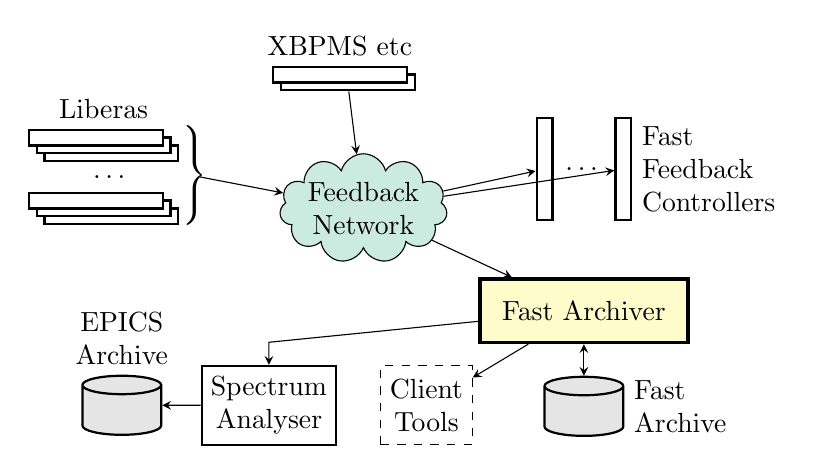
\begin{tikzpicture}

% Nice puffy cloud representing the FA network
\path[xshift=27mm, yshift=5mm, thin]
    node[draw, cloud, aspect=2, cloud puffs=11, inner sep=0pt, highlight fill,
        align=center]
        (fa network) {Feedback\\Network};

% Draw a stack of rectangles representing the liberas
\path[xshift=-5mm, yshift=12mm,
    libera/.style={
        draw, rectangle, thick, fill=white, inner sep=0,
        minimum width=1.7cm, minimum height=2mm}]

    { [current point is local=true]
    node[libera] {}
    ++(-1mm,1mm) node[libera] {}
    ++(-1mm,1mm) node[libera] (top libera) {}
    }

    +(0mm,-3mm) node {\dots}
    ++(0mm,-8mm)
    { [current point is local=true]
    node[libera] (bottom libera) {}
    ++(-1mm,1mm) node[libera] {}
    ++(-1mm,1mm) node[libera] {}
    }
    node[tight fit=(top libera) (bottom libera),
        right delimiter=\}, label=north:Liberas] (liberas) {};

\draw[->] ($(liberas.east)+(2.6mm,0)$) -- (fa network);

\path[xshift=25mm, yshift=21mm,
    libera/.style={
        draw, rectangle, thick, fill=white, inner sep=0,
        minimum width=1.7cm, minimum height=2mm}]

    node[libera] (xbpms) {}
    ++(-1mm,1mm) node[libera, label=north:XBPMS etc] {};

\draw[->] (xbpms) -- (fa network);


% Fast feedback controllers
\path[xshift=50mm, yshift=10mm,
    controller/.style={
        draw, rectangle, thick, inner sep=0,
        minimum width=2mm, minimum height=13mm}]

    node[controller] (left controller) {}
    ++(5mm,0mm) node {\dots}
    ++(5mm,0mm) node[controller,
        label={[align=left]right:Fast\\Feedback\\Controllers}]
    (right controller) {};

\draw[->] (fa network) -- (left controller);
\draw[->] (fa network) -- (right controller);

% The archiver saving into the archive store
\path[xshift=5.5cm, yshift=-8mm]
    node[draw, very thick, rectangle, inner sep=8pt, fill=yellow!20]
        (archiver) {Fast Archiver}

    node[disk icon, below=4mm of archiver, fill=black!10] (fa archive) {}
    node[tight fit=(fa archive),
        label={[align=left]right:Fast\\Archive}] {}
    [draw,<->] (archiver) -- (fa archive);

\draw[->] (fa network) -- (archiver);

% Spectrum analyser saving into EPICS archive
\path[xshift=15mm, yshift=-20mm]
    node[draw, thick, rectangle, align=center, minimum height=10mm]
        (spectrum) {Spectrum\\Analyser}

    node[disk icon, anchor=shape center, fill=black!10,
        label={[align=center]above:EPICS\\Archive}]
        (epics archive) at ($(spectrum.west)-(10mm,0)$) {}
    node[tight fit=(epics archive)] (epics archive fit) {}

    [draw,->] (spectrum) -- (epics archive fit);

\draw[->] (archiver) -- ($(spectrum)+(0,8mm)$) -- (spectrum);

% Client tools
\path[xshift=35mm, yshift=-20mm]
    node[draw, rectangle, align=center, minimum height=10mm, dashed]
        (client tools) {Client\\Tools};

\draw[->] (archiver) -- (client tools);

\end{tikzpicture}

% vim: set filetype=tex:

\end{center}
\end{frame}



\begin{frame}\frametitle{Data Sources and Sinks}
Data Sources:
\begin{itemize}
\item Libera Electron Beam Position Monitors (174)
\item X-Ray Beam Position Monitors (28)
\item RF cavity monitors (2)
\item Accelerometer (1)
\end{itemize}
\vskip1ex
Data Sinks:
\begin{itemize}
\item \texttt{fa-viewer} for live data
\item \texttt{fa\_zoomer} for viewing historical data
\item \texttt{matlab} and \texttt{fa\_load} for analysing historical data
\item Spectrum analyser
\item Other tools to be added over time \dots
\end{itemize}
\end{frame}



\begin{frame}\frametitle{FA Archiver Architecture}

\begin{itemize}

\item Very regular data feed: fixed size updates at fixed intervals.
Makes archiver design much simpler than an EPICS archiver.

\item The historical archive is fixed length, determined by disk size.  Old data
is discarded as new data arrives.

\item Data is reordered for fast read access before storage to disk.

\item File system overhead is avoided by storing archiver database on raw block
device!

\item Overview data (decimated by binning) also stored.

\item Archive indexed by timestamp of arrival of CC data.

\end{itemize}
\end{frame}



\begin{frame}\frametitle{FA Archiver Architecture}
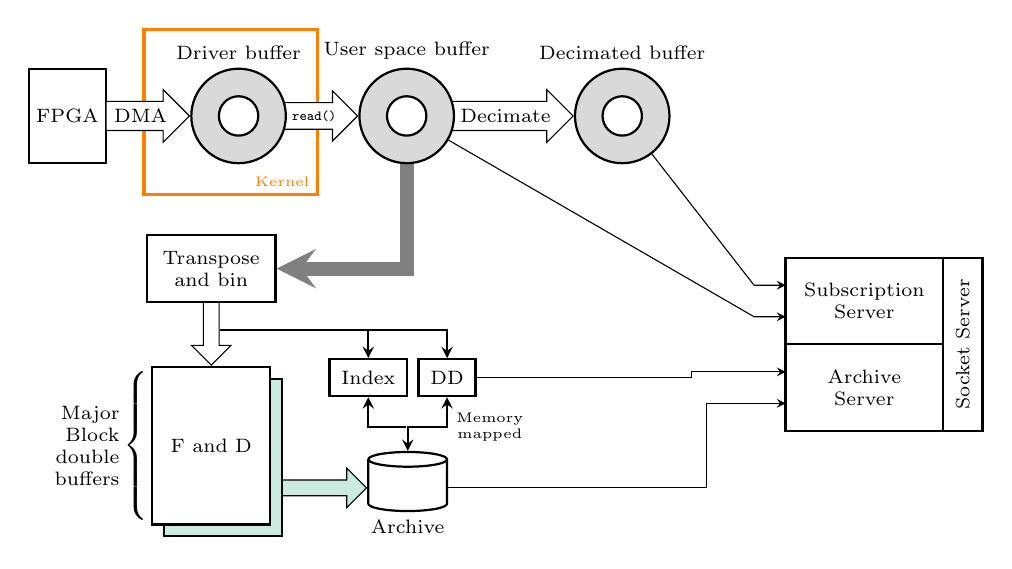
\begin{tikzpicture}[
    single arrow head extend=1.5mm]
\scriptsize

% Draws a circular buffer with name #1 east of #2 with top label #3 and centre
% label #4
\newcommand{\buffer}[3]{
\begin{pgfonlayer}{foreground}
\path
    node [draw, thick, circle, background fill,
        minimum width=12mm, anchor=west,
        label={above:#3}] (#1) at (#2.east) {}
    node [draw, thick, fill=white, circle, minimum width=5mm] at (#1) {};
\end{pgfonlayer}
}

% Sniffer device and its connections
\node [draw, thick, anchor=west, minimum height=12mm] (fpga) {FPGA};
\node [draw, single arrow, anchor=west, fill=white]
    (dma) at ($(fpga.east)-(0.2mm,0)$) {DMA};

% Device driver
\buffer{device buffer}{dma}{Driver buffer}
\node [draw, single arrow, anchor=west, fill=white]
    at ($(device buffer.east)-(0.4mm,0)$)
    (device) {\tiny\texttt{read()}};

\begin{pgfonlayer}{background}
\draw [orange, very thick] ($(device buffer)+(-12mm,11mm)$)
    rectangle ($(device buffer)+(10mm,-10mm)$);
\node [orange, anchor=south east, font=\tiny]
    at ($(device buffer)+(10mm,-10mm)$) {Kernel};
\end{pgfonlayer}


% Central raw circular buffer and decimated buffer
\buffer{raw buffer}{device}{User space buffer}
\node [draw, single arrow, anchor=west] at ($(raw buffer.east)-(0.4mm,0)$)
    (decimate) {Decimate};
\buffer{decimated buffer}{decimate}{Decimated buffer}


% Transposing to in-memory disk buffer
\node [draw, thick, anchor=north west, inner sep=2mm, align=center]
    at (15mm, -15mm)
    (transpose) {Transpose\\and bin};
\path [draw, line width=5pt, color=gray, ->] (raw buffer) |- (transpose);
\node [draw, single arrow, rotate=-90, anchor=west, minimum height=8mm]
    (transpose arrow) at ($(transpose.south)+(0,0.2mm)$) {};
\begin{pgfonlayer}{foreground}
\node [draw, thick, fill=white,
    minimum height=20mm, minimum width=15mm, anchor=north, align=center,
    left delimiter=\{, copy shadow={
        shadow xshift=1.5mm, shadow yshift=-1.5mm, highlight fill},
    label={[align=right, xshift=-3mm]left:Major\\Block\\double\\buffers}]
    (major block) at (transpose arrow.east) {F and D};
\end{pgfonlayer}


% Archive on disk and in memory
\node [draw, single arrow, anchor=west, minimum width=1mm, minimum height=12mm,
    highlight fill]
    (archive arrow) at (major block.325) {};
\node [disk icon, anchor=west, label={below:Archive}]
    (archive) at (archive arrow.east) {};

\node [draw, thick, inner sep=1.5mm]
    (index) at ($(archive)+(-5mm,14mm)$) {Index};
\node [draw, thick, inner sep=1.5mm] (dd) at ($(archive)+(+5mm,14mm)$) {DD};

\draw [->, thick] (transpose arrow) -| (index);
\draw [->, thick] (transpose arrow) -| (dd);
\node [inner sep=0pt, line width=0] (via) at ($(archive.north)+(0,3mm)$) {};
\draw [<-, thick] (index) |- (via);
\draw [<->, thick] (dd) |- (via.center) -- (archive);

\node [right=5mm of via, align=center, font=\tiny] {Memory\\mapped};


% Socket Server
\path [draw, thick]
    (\linewidth, -40mm) rectangle ++(-5mm,22mm) coordinate (a)
    node [rotate=90, pos=0.5] {Socket Server}
    rectangle ++(-20mm,-11mm) coordinate (b)
    node [pos=0.5, align=center] {Subscription\\Server}
    rectangle ++(20mm,-11mm) coordinate (c)
    node [pos=0.5, align=center] {Archive\\Server}
    node [tight fit=(a) (b), align=center] (subscription server) {}
    node [tight fit=(b) (c), align=center] (archive server) {};

\draw [<-] ($(subscription server.west)+(0,-2mm)$)
    -- +(-4mm,0) -- (raw buffer);
\draw [<-] ($(subscription server.west)+(0,2mm)$)
    -- +(-4mm,0) -- (decimated buffer);
\draw [<-] ($(archive server.west)+(0,2mm)$) -- +(-12mm,0) |- (dd);
\draw [<-] ($(archive server.west)+(0,-2mm)$) -- +(-10mm,0) |- (archive);


\end{tikzpicture}

% vim: filetype=tex:

\end{frame}


\begin{frame}\frametitle{Archive Index}
Structure of index can be extremely simple.
\begin{itemize}
\item FA data is gathered into blocks of 65536 samples or around 6.5 seconds
each.
\item The timestamp of the first sample in each block is stored, together with
its duration and a communication controller timestamp, referred to as ``id0''.
\item Search for offset of block with desired timestamp by binary search of
index --- very fast as index is small.  {\scriptsize(16 probes)}
\item All timestamps internally stored as 64-bit counts of microseconds in the
Unix (UTC) epoch --- we're good for \textonehalf{} million years!
\item Index operates as a circular buffer: new data overwrites old.
\end{itemize}
\end{frame}


\begin{frame}\frametitle{Data Transformation}
\begin{itemize}
\item Data arrives interleaved (N = 256 or 512):
\[
\begin{matrix}
xy_{0,t}   & xy_{1, t}   & \cdots & xy_{N-1,t} \\
xy_{0,t+1} & xy_{1, t+1} & \cdots & xy_{N-1,t+1} \\
\vdots & \vdots & \cdots & \vdots
\end{matrix}
\]
\item Desperately inefficient to access in this sequence
\item Data for each ID gathered into long blocks for writing:
\[
\begin{matrix}
xy_{0,t} & \cdots & xy_{0,t+T-1} \\
xy_{1,t} & \cdots & xy_{1,t+T-1} \\
\vdots & \vdots & \vdots \\
xy_{N-1,t} & \cdots & xy_{N-1,t+T-1} \\
xy_{0,t+T} & \cdots & xy_{0,t+2T-1} \\
\vdots & \vdots & \vdots \\
\end{matrix}
\qquad T = 65536
\]
\item This transposing is essential for performance
\end{itemize}

% Highlights above, found by stabs in the dark!  Alas, the background layer
% still seems to come after ordinary text, so we need to use opacity instead.
\begin{tikzpicture}[overlay]
\path [fill=black, opacity=0.1]
    (current page.north west) ++(30mm,-25mm) [fill] rectangle ++(60mm,5mm);
\path [fill=black, opacity=0.1]
    (current page.north west) ++(22mm,-73mm) [fill] rectangle ++(18mm,22mm);
\path [fill=green!60!blue, opacity=0.2]
    (current page.north west) ++(22mm,-56mm) [fill] rectangle ++(50mm,5mm);
\end{tikzpicture}
\end{frame}


\begin{frame}\frametitle{Decimated Archive Data}
To help with reviewing beam movement over hours or days, the archived data is
also stored in decimated format.
\begin{itemize}
\item Two degrees of decimation: $\div 128$ (approx 80\,Hz) and $\div 16384$
(approx 1\textonehalf{} seconds per sample): ``single'' and ``double'' decimated
data.
\item Archived decimation is by binning; for each bin the archiver stores: mean,
minimum, maximum and standard deviation:
\[
\overline{x}, \lfloor x\rfloor, \lceil x\rceil, \sigma_x
\qquad\text{and}\qquad
\overline{y}, \lfloor y\rfloor, \lceil y\rceil, \sigma_y
\quad.
\]
\item A fortnight of data for one data source can be previewed with a 750,000
point waveform, rather than 12,000,000,000 points!
\end{itemize}
\end{frame}


\begin{frame}\frametitle{Binned Archive Data}
\begin{center}
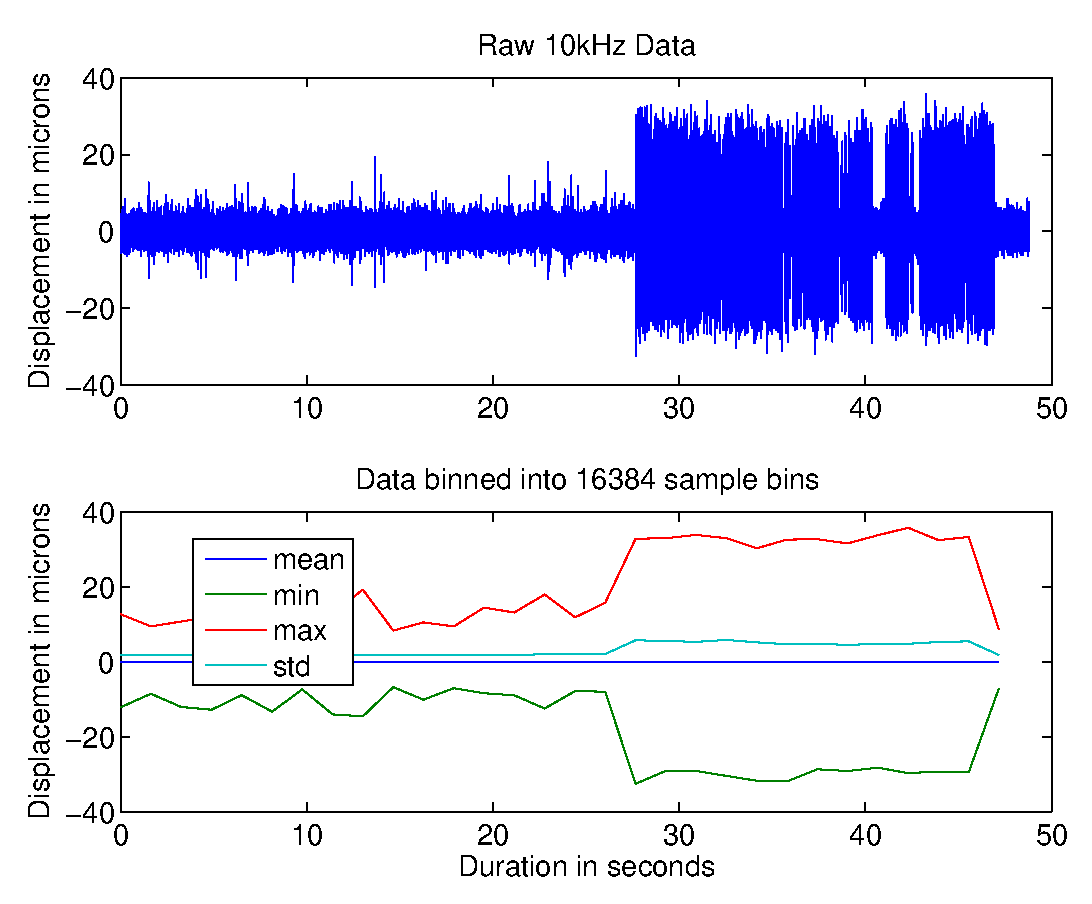
\includegraphics[width=.9\linewidth]{binning}
\end{center}
\end{frame}


\begin{frame}\frametitle{Archive Database Layout}
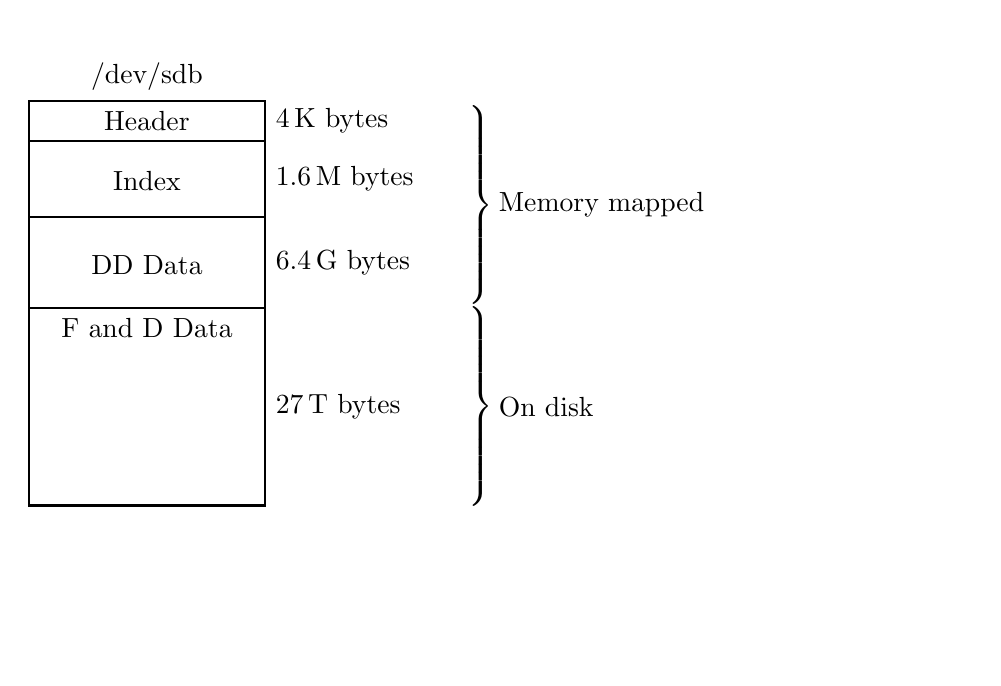
\begin{tikzpicture}

% Common database layout

\path % [draw, thick]
    (-40mm,-45mm) rectangle (80mm,35mm) {};

\node [
    rectangle split, rectangle split parts=4, draw, thick,
    minimum width=30mm, anchor=west,
    label={above:/dev/sdb}] (disk) at (-40mm,0)
    {
        Header
    \nodepart{two}
        Index\rule[-2mm]{0pt}{7mm}
    \nodepart{three}
        DD Data\rule[-3mm]{0pt}{9mm}
    \nodepart{four}
        F and D Data\rule[-20mm]{0pt}{0pt}
    };

% vim: filetype=tex:



\node [anchor=west] at (disk.text east) {4\,K bytes};
\node [anchor=west] at (disk.two east) {1.6\,M bytes};
\node [anchor=west] at (disk.three east) {6.4\,G bytes};
\node [anchor=west] at (disk.four east) {27\,T bytes};


\node [inner sep=0] (text corner) at ($(disk.three split east)+(25mm,0)$) {};
\node [
    fit=(disk.north east) (text corner),
   % fit=(header size) (index size) (dd size),
    inner sep=0, right delimiter=\},
    label={[xshift=3mm]right:Memory mapped}] {};
\node [fit=(text corner) (disk.south east),
    inner sep=0, right delimiter=\},
    label={[xshift=3mm]right:On disk}] {};

\end{tikzpicture}

% vim: filetype=tex:

\end{frame}


\begin{frame}\frametitle{Archive Database Layout: Header}
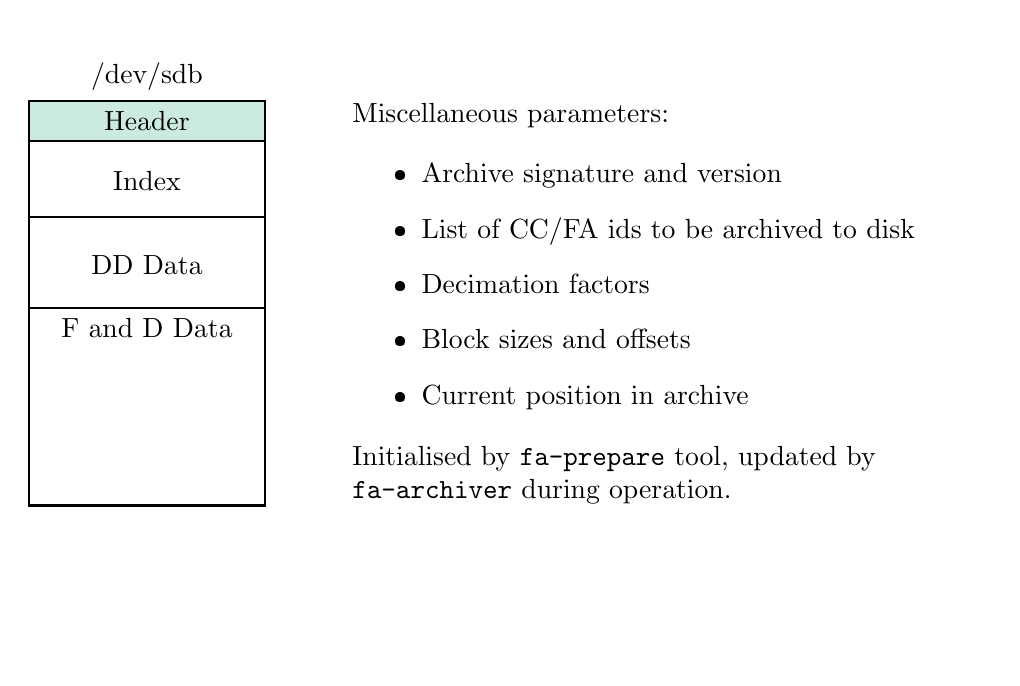
\begin{tikzpicture}

% Common database layout

\path % [draw, thick]
    (-40mm,-45mm) rectangle (80mm,35mm) {};

\node [
    rectangle split, rectangle split parts=4, draw, thick,
    minimum width=30mm, anchor=west,
    label={above:/dev/sdb}] (disk) at (-40mm,0)
    {
        Header
    \nodepart{two}
        Index\rule[-2mm]{0pt}{7mm}
    \nodepart{three}
        DD Data\rule[-3mm]{0pt}{9mm}
    \nodepart{four}
        F and D Data\rule[-20mm]{0pt}{0pt}
    };

% vim: filetype=tex:


\begin{pgfonlayer}{background}
\path [highlight fill] (disk.north west) rectangle (disk.text split east);
\end{pgfonlayer}

\node [anchor=west, text width=80mm] {
Miscellaneous parameters:

\begin{itemize}
\item Archive signature and version
\item List of CC/FA ids to be archived to disk
\item Decimation factors
\item Block sizes and offsets
\item Current position in archive
\end{itemize}

Initialised by \texttt{fa-prepare} tool, updated by \texttt{fa-archiver} during
operation.
};


\end{tikzpicture}

% vim: filetype=tex:

\end{frame}


\begin{frame}\frametitle{Archive Database Layout: Index}
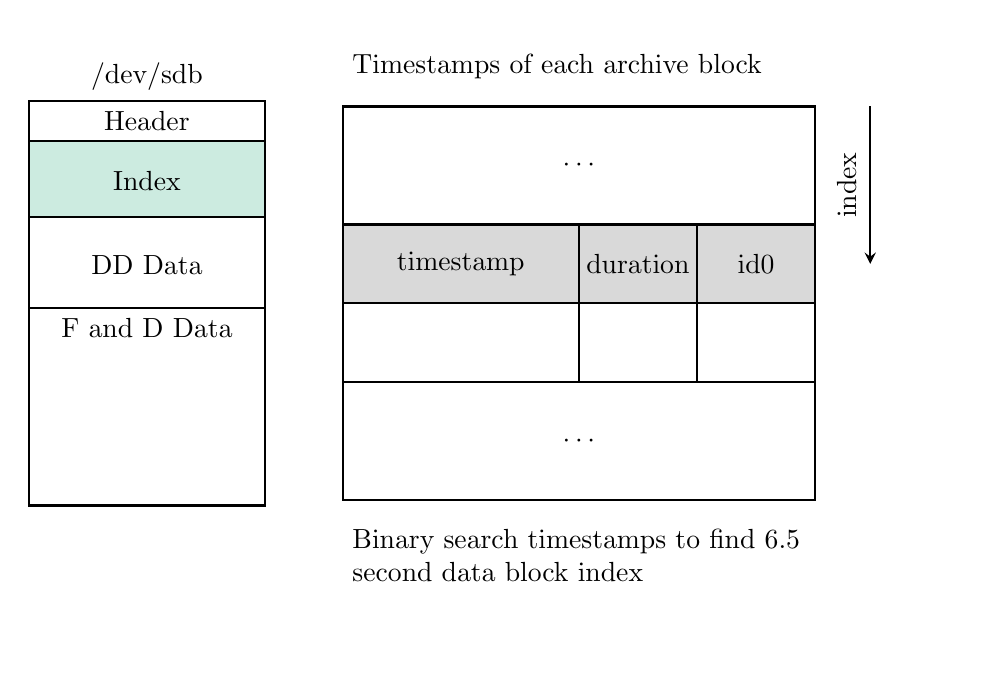
\begin{tikzpicture}

% Common database layout

\path % [draw, thick]
    (-40mm,-45mm) rectangle (80mm,35mm) {};

\node [
    rectangle split, rectangle split parts=4, draw, thick,
    minimum width=30mm, anchor=west,
    label={above:/dev/sdb}] (disk) at (-40mm,0)
    {
        Header
    \nodepart{two}
        Index\rule[-2mm]{0pt}{7mm}
    \nodepart{three}
        DD Data\rule[-3mm]{0pt}{9mm}
    \nodepart{four}
        F and D Data\rule[-20mm]{0pt}{0pt}
    };

% vim: filetype=tex:


\node [anchor=west] at +(0,30mm)
    {Timestamps of each archive block};


\path [draw, thick]
    (60mm,-25mm) rectangle ++(-60mm,50mm)
    rectangle ++(60mm,-15mm)
    node [pos=0.5, align=center] {$\cdots$}
    coordinate (a) {}
    rectangle ++(-15mm,-10mm)
    node [pos=0.5, align=center] {id0}
    rectangle ++(-15mm,10mm)
    node [pos=0.5, align=center] {duration}
    rectangle ++(-30mm,-10mm)
    coordinate (b) {}
    node [pos=0.5, align=center] {timestamp}
    rectangle ++(30mm,-10mm) rectangle ++(15mm,10mm) rectangle ++(15mm,-10mm)
    rectangle ++(-60mm,-15mm)
    node [pos=0.5, align=center] {$\cdots$};

\node [anchor=west, text width=60mm] at (0,-32mm)
    {Binary search timestamps to find 6.5 second data block index};

\path [draw, ->, thick] (67mm,25mm) -- ++(0mm,-20mm)
    node [pos=0.5, align=center, rotate=90, yshift=3mm] {index};


\begin{pgfonlayer}{background}
\path [highlight fill] (disk.text split west) rectangle (disk.two split east);
\draw [background fill] (a) rectangle (b);
\end{pgfonlayer}


\end{tikzpicture}

% vim: filetype=tex:

\end{frame}


\begin{frame}\frametitle{Archive Database Layout: Double Decimated Data}
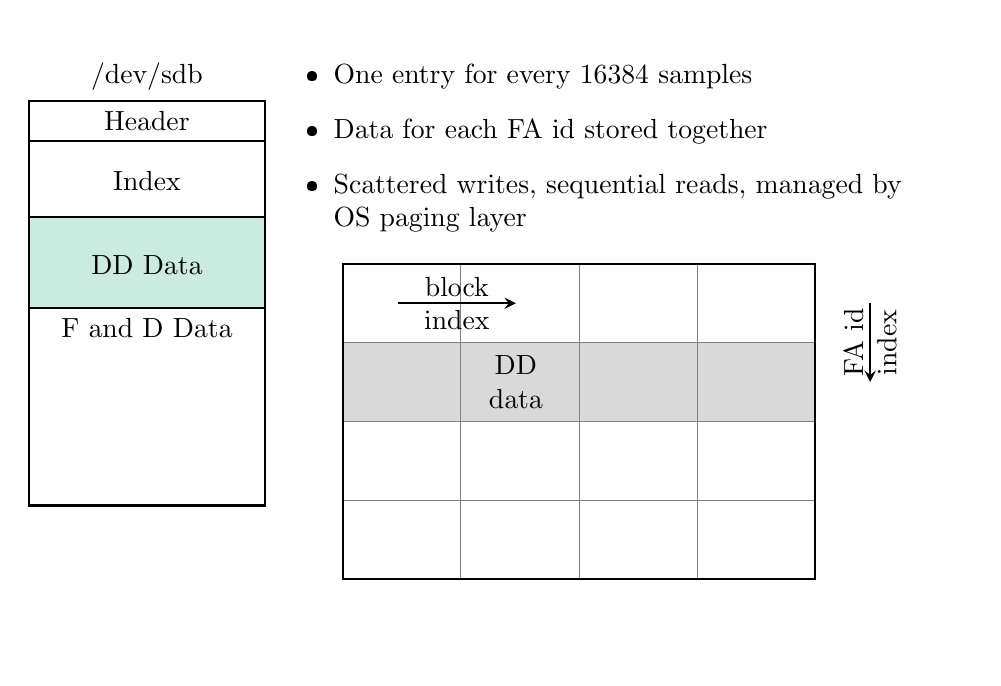
\begin{tikzpicture}

% Common database layout

\path % [draw, thick]
    (-40mm,-45mm) rectangle (80mm,35mm) {};

\node [
    rectangle split, rectangle split parts=4, draw, thick,
    minimum width=30mm, anchor=west,
    label={above:/dev/sdb}] (disk) at (-40mm,0)
    {
        Header
    \nodepart{two}
        Index\rule[-2mm]{0pt}{7mm}
    \nodepart{three}
        DD Data\rule[-3mm]{0pt}{9mm}
    \nodepart{four}
        F and D Data\rule[-20mm]{0pt}{0pt}
    };

% vim: filetype=tex:


\begin{pgfonlayer}{background}
\path [highlight fill] (disk.two split west) rectangle (disk.three split east);
\path [background fill] (0,-15mm) rectangle (60mm,-5mm);
\end{pgfonlayer}

\node [anchor=west, inner sep=0, text width=85mm] at +(-10mm,22mm)
{
\begin{itemize}
\item One entry for every 16384 samples
\item Data for each FA id stored together
\item Scattered writes, sequential reads, managed by OS paging layer
\end{itemize}
};


\draw [help lines, yshift=5mm]
    (0,-40mm) grid[draw, xstep=15mm, ystep=10mm] ++(60mm,40mm);
\path [draw, thick]
    (0,5mm) rectangle ++(60mm,-40mm);
\draw [thick, ->] (7mm,0) -- +(15mm,0)
    node [pos=0.5, align=center] {block\\index};
\node [align=center] at (22mm,-10mm) {DD\\data};
\draw [thick, ->] (67mm,0) -- +(0,-10mm)
    node [pos=0.5, align=center, rotate=90] {FA id\\index};


\end{tikzpicture}

% vim: filetype=tex:

\end{frame}


\begin{frame}\frametitle{Archive Database Layout: FA Data}
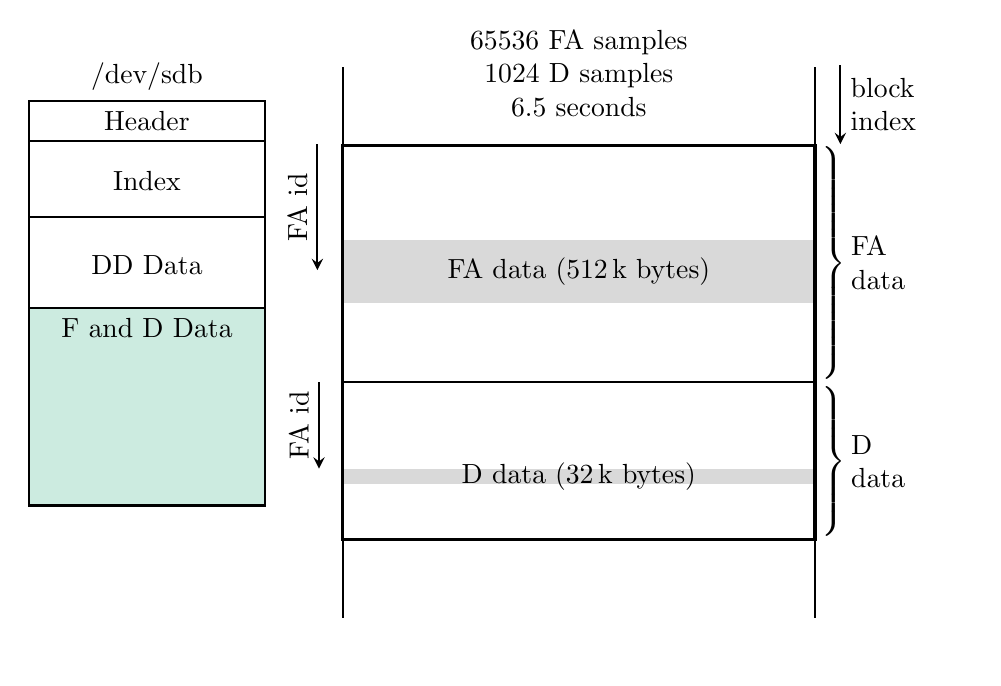
\begin{tikzpicture}

% Common database layout

\path % [draw, thick]
    (-40mm,-45mm) rectangle (80mm,35mm) {};

\node [
    rectangle split, rectangle split parts=4, draw, thick,
    minimum width=30mm, anchor=west,
    label={above:/dev/sdb}] (disk) at (-40mm,0)
    {
        Header
    \nodepart{two}
        Index\rule[-2mm]{0pt}{7mm}
    \nodepart{three}
        DD Data\rule[-3mm]{0pt}{9mm}
    \nodepart{four}
        F and D Data\rule[-20mm]{0pt}{0pt}
    };

% vim: filetype=tex:


\begin{pgfonlayer}{background}
\path [highlight fill] (disk.three split west) rectangle (disk.south east);
\end{pgfonlayer}

\begin{pgfonlayer}{foreground}
\draw [very thick] (0,20mm)
    coordinate (a) {} rectangle (60mm,-30mm)
    coordinate (b) {} node[fit=(a) (b), inner sep=0] (fa data) {};
\end{pgfonlayer}

\node [text width=60mm, align=center]
    at (30mm,28mm) {\smash{65536 FA samples}\\1024 D samples\\6.5 seconds};
\path [thick]
    (0,30mm) [draw] -- (0,-40mm)
    (60mm,30mm) [draw] -- (60mm,-40mm);
\draw [thick] (0,-10mm) -- (60mm,-10mm) coordinate (sep) {};
\node [fit=(fa data.north east) (sep), right delimiter=\}, inner sep=0,
    label={[align=left, xshift=3mm]right:FA\\data}] {};
\node [fit=(fa data.south east) (sep), right delimiter=\}, inner sep=0,
    label={[align=left, xshift=3mm]right:D\\data}] {};

\path
    (fa data.north east) ++(3mm,0)
    [draw, thick, <-] -- ++(0, 10mm)
    node [pos=0.5, align=left, anchor=west] {block\\index};

\fill [background fill]
    (0,0) rectangle ++(60mm,8mm)
    node [pos=0.5, black] {FA data (512\,k bytes)};
\path
    (fa data.north west) ++(-3mm,0)
    [draw, thick, ->] -- ++(0,-16mm)
    node [pos=0.5, rotate=90, anchor=south] {FA id};

\fill [background fill]
    (0,-23mm) rectangle ++(60mm,2mm)
    node [pos=0.5, black] {D data (32\,k bytes)};
\path
    (0,-10mm) ++(-3mm,0)
    [draw, thick, ->] -- ++(0,-11mm)
    node [pos=0.5, rotate=90, anchor=south] {FA id};



\end{tikzpicture}

% vim: filetype=tex:

\end{frame}



\begin{frame}\frametitle{Archiver Services}

The FA archiver provides the following data over TCP/IP to any connecting
machine:

\begin{itemize}

\item Subscription to any subset of the complete CC data stream.
\note{If the client doesn't take data rapidly enough it will be disconnected by
the server.}

\item Subscription to any subset of the complete CC data stream decimated by
filtering by a factor of 10.

\item Access to any part of the historical archive, both full and decimated,
indexed by timestamp.

\end{itemize}
\end{frame}



\begin{frame}\frametitle{Filtered Decimated Data}
\begin{itemize}
\item The entire FA data stream is decimated by filtering by a factor of 10 down
to 1\,kHz
\item This is independent of binned archive decimated data
\item Designed to assist whole orbit analysis, reduces data rate
\item Filtering performed by ``Compensated Cascaded Integrater Comb'' (CIC).
Fast to implement with very good spectral behaviour: effectively flat to
400\,Hz.
\end{itemize}
\begin{center}
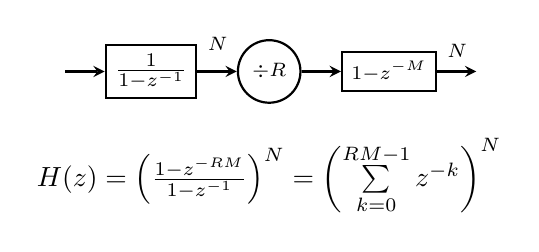
\begin{tikzpicture} [start chain, node distance=5mm, thick, ->]

\node [on chain, join] {};
\node [on chain, join, draw] (I) {$\frac1{1-z^{-1}}$};
\node [on chain, join, draw, circle] (R) {$\scriptstyle\div R$};
\node [on chain, join, draw] (D) {$\scriptstyle1-z^{-M}$};
\node [on chain, join] {};

\node [anchor=west] at (I.north east) {$\scriptstyle N$};
\node [anchor=west] at (D.north east) {$\scriptstyle N$};

\node [anchor=north, yshift=-3mm] at (R.south)
    {$H(z) = \left(\frac{1-z^{-RM}}{1-z^{-1}}\right)^N
        = \left(\sum\limits_{k=0}^{RM-1}z^{-k}\right)^N$};

\end{tikzpicture}

% vim: filetype=tex:

\end{center}
\end{frame}


\begin{frame}\frametitle{Filtered Decimated Data}
\begin{center}
\includegraphics[width=0.8\linewidth]{filter}
\end{center}
\end{frame}



\begin{frame}\frametitle{Spectrum Analysis Tool}
\begin{center}
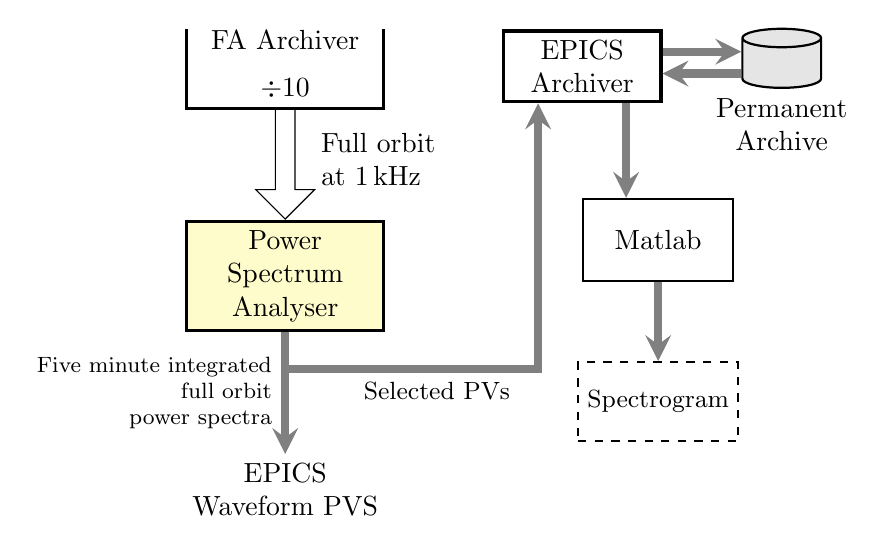
\begin{tikzpicture}

\draw [very thick]
    (0,0) coordinate(ar-nw) -- ++(0,-10mm) --
    ++(25mm,0) coordinate[midway] (ar-s) -- ++(0,10mm) coordinate(ar-ne);
\node [anchor=north, inner sep=0pt] at ($(ar-nw)!.5!(ar-ne)$) {FA Archiver};
\node [anchor=south] at (ar-s) {$\div 10$};

\node [draw, single arrow, rotate=-90, anchor=west, minimum height=14mm,
    label={[align=left, xshift=2mm]above:Full orbit\\at 1\,kHz}]
    (from-archiver) at (ar-s) {};
\node [draw, very thick, anchor=north, align=center, minimum width=25mm,
    fill=yellow!20]
    (analyser) at (from-archiver.east) {Power\\Spectrum\\Analyser};

\node [align=center] (pvs)
    at ($(analyser.south)+(0,-20mm)$) {EPICS\\Waveform PVS};
\draw [gray, line width=3pt, ->] (analyser) -- (pvs)
    coordinate[pos=0.3] (pv nw)
    node [anchor=east, pos=0.5, black, align=right, font=\footnotesize]
    {Five minute integrated\\full orbit\\power spectra};

\node [draw, very thick, align=center, anchor=north west, minimum width=20mm]
    (epics ar) at (40mm,0) {EPICS\\Archiver};
\node [disk icon, anchor=west, xshift=10mm, fill=black!10,
    label={[align=center]below:Permanent\\Archive}]
    (disk) at (epics ar.east) {};
\draw [gray, line width=3pt, ->] (disk.160 -| epics ar.east) -- (disk.160);
\draw [gray, line width=3pt, <-] (disk.190 -| epics ar.east) -- (disk.190);

\draw [gray, line width=3pt, ->] (pv nw) -| (epics ar.-140)
    node [pos=0.3, black, below, font=\small] {Selected PVs};


\node [draw, thick, anchor=north west, inner sep=4mm, yshift=-12mm]
    (matlab) at (epics ar.south) {Matlab};
\draw [gray, line width=3pt, ->]
    (epics ar.-40) -- (epics ar.-40 |- matlab.north);

\node [draw, thick, anchor=north, yshift=-10mm, font=\small, dashed,
    minimum height=10mm]
    (figure) at (matlab.south) {Spectrogram};
\draw [gray, line width=3pt, ->] (matlab) -- (figure);


\end{tikzpicture}

\end{center}
\end{frame}


\begin{frame}\frametitle{Spectrum Analysis Tool: EDM Screen}
\begin{center}
\includegraphics[height=80mm]{spectrum}
\end{center}
\end{frame}


\begin{frame}\frametitle{Spectrogram at one EBPM for a Week}
\includegraphics[width=\linewidth]{spectrogram-3-2}
\end{frame}



\begin{frame}\frametitle{FA Zoomer Matlab Interface}
\includegraphics[width=\linewidth]{fa-zoomer}
\end{frame}


\begin{frame}\frametitle{FA Viewer}
\begin{center}
\includegraphics[width=.85\linewidth]{WEPMN004f6}
\end{center}
\end{frame}


\begin{frame}\frametitle{Allan Variance from the Archive}
\begin{itemize}
\item Allan Variance developed for assessing stability of oscillators and clocks
\item Generally useful for assessing stability in general over many orders of
magnitude in time
\item Also called ``two sample variance'', difference of adjacent averages
($\tau$ = sample duration):
\begin{gather*}
\sigma_y^2(\tau) =
    \frac12\langle(\overline{y}_{i+1} - \overline{y}_i)^2\rangle \\[1ex]
\overline{y}_i = \frac1\tau \int_0^\tau y(i\tau + t) \, dt
\end{gather*}
\item Can use FA archive to cover dynamic range 10\,kHz to around
1\,\textmu{}Hz (ten orders of magnitude).
\end{itemize}
\end{frame}


\begin{frame}\frametitle{Example Application of Allan Variance}
\includegraphics[width=\linewidth]{allan}
\end{frame}


\begin{frame}\frametitle{Lessons Learned}
\begin{itemize}
\item Buffer sizes matter:
    \begin{itemize}
    \item 512\,K seems a sweet spot for disk access
    \item perhaps 64\,K for network access?
    \end{itemize}
\item Modern processors can do floating point \emph{very} fast
\item Integer to floating point conversion is \emph{sloooow}!
\item \texttt{valgrind} can find very elusive bugs
\end{itemize}
\end{frame}


\begin{frame}\frametitle{Lessons for a New EPICS Archiver?}
\begin{itemize}
\item Write patterns and read patterns are very different: archiver should
optimise for readers by gathering data together over time for each PV.
\item Important to avoid scattered disk access for performance
\item Aggregated decimation (mean/min/max/variance) is very helpful for data
overview.
\end{itemize}
I suggest a novel EPICS archiver architecture which captures complete history of
\emph{all} PVs (within reason) over a limited history, and then decimates and
aggregates for long term history, possibly on a constant 1 minute tick.
\end{frame}


% How to skip a block of (valid) code:
\iffalse \fi

\end{document}
